\chapter{Contribuição}\label{meto}

A contribuição dessa pesquisa é de cunho metodológico-prático.
Do ponto de vista metodológico, pela aplicação do processo CRISP-DM, usado para construir o modelo preditivo e classificativo; pela integração entre mineração de dados históricos e mineração de textos; pela utilização de algoritmos de classificação e de predição. 

No que diz respeito à mineração de dados, as técnicas de classificação utilizadas foram Árvores de Decisão e Naïve Bayes. Quanto às técnicas de predição, utilizou-se Redes Neurais (regressão logística, como caso particular). Para mineração de textos foi utilizado o Text frequency - Inverse Document Frequency (TF-IDF).

Do ponto de vista prático, pela proposição de um modelo que integre predição à API de mapas de posicionamento global, fornecendo informação suficiente para um utilizador tomar uma decisão acerca dos dias e horários que ofereçam menor risco de acidentes ou qualquer evento que implique na retenção do fluxo de veículos. 

As soluções disponíveis que existem, tais como; Google Maps, Waze e outras ferramentas dessa natureza somente exibem, até o momento dessa pesquisa, informações momentâneas, produzidas e compartilhadas pelos utilizadores dos aplicativos, ou por informações provindas de GPS. Contudo, não analisam dados históricos dessas rodovias, nem fazem predições sobre o seu comportamento.

Outra contribuição dessa pesquisa é a proposição de um arco cibernético construído com a API de redes sociais.
Os ``feeds'' de notícias das redes sociais como o Twitter permitem analisar o contexto das rodovias com defasagem temporal muito pequena.
Os utilizadores dessas redes sociais contribuem com informações relevantes como, por exemplo, o anúncio de uma paralisação que ocorrerá 
daqui a alguns dias. A PRF de Pernambuco é outro contribuidor permanente. Com seu canal no Twitter: @PRF191PE, fornece diariamente informação das rodovias, 
além de dados estatísticos relativos a acidentes e retenção de tráfego, como aqueles decorrentes de protestos, que, quando feitos dentro da lei
devem ser informados à PRF, com dia e hora marcados antecipadamente.

A monitoração de redes sociais foi feita a partir de Mineração em Textos - Knowldge Database Text (KDT), tendo, a princípio, sido executada no Twitter, no canal PRF191PE e pela busca em outros canais, com as palavras: ''protesto´´, ''planejar paralização'', por exemplo. 

Para ter-se acesso aos tweets da PRF, os usuários do canal, inclusive a própria PRF, postam comentários diretamente 
na API do Twitter ou por um navegador. Para essa pesquisa as palavras-chave tais como: protestos, acidentes, paralisação, foram de suma importância.

Uma vez capturados, esses tweets foram tratados por Mineração em Textos e analisados instantaneamente por algoritmos de I.A. 
A técnica utilizada para análise dos textos foi a análise de palavras ou termos frequentes (TDF-IDF). O algoritmo de classificação escolhido foi Naïve Bayes, por ser um classificador rápido e eficiente, e por ter sido utilizado na primeira fase dessa pesquisa, servindo como comparativo à Árvore de Decisão. O algoritmo de agrupamento (clustering) foi o K-means.



\section{Modelo Proposto}

A metodologia utilizada nessa pesquisa contempla um plano em três etapas, cada uma dividida em fases atinentes.
A primeira etapa da nossa metodologia contempla todas as fases do CRISP-DM, onde está o modelo classificativo, o preditivo e 
a descoberta de conhecimento sobre o comportamento das rodovias estudadas. A descoberta de conhecimento sobre esse comportamento 
 tem a ver com o ``modus operandi'' dos seus utilizadores. A priori, especulou-se sobre possíveis erros de traçados e outros que pudessem
ser identificados pelos algoritmos de mineração empregados no processo.

Os algoritmos escolhidos contemplaram algumas características especiais, tais como, robustez, tolerância à faltas (missing data),
taxa de aprendizagem e facilidade de interpretação dos dados processados. 

No quesito tolerância à faltas e facilidade de interpretação dos dados, a Árvore de Decisão e o Naïve Bayes se destacaram por não necessitar
de qualquer requisito extra para entender e interpretar os resultados.

No quesito robustez, tolerância à faltas e taxa de aprendizagem relativamente alta, as redes neurais artificiais (RNA), com a 
topologia Perceptron multicamadas com retroalimentação ``backpropagation'', se destacaram por terem adequada capacidade de generalização e especificidade em modelos de predição. 

A extrapolação do modelo preditivo deverá ocorrer quando este se integrar a uma estrutura dinâmica, composta pela redes sociais e mapas vetoriais, dado um espaço temporal pré-determinado por um agente: o utilizador. 

Através de API's, os mapas vetoriais permitem a geolocalização dos pontos classificados ou pontos onde haverá grande número de retenções, conhecido como \textbf{gargalo}.

Para a integração às redes sociais, foi escolhida a API do Twitter. Esta ``interface'' é simples de ser configurada. A quantidade de informações produzidas pelos utilizadores gera poucos dados em cada postagem, mas é eficaz. O utilizador tem que ser sucinto ao publicar suas postagem em um espaço de 140 caracteres. Isso facilita a forma como os dados são extraídos pela quantidade diminuta, bem como a quantidade de conexões à Internet. Contudo, esta rede social tem uma crescente quantidade de postagens no formato imagens, dificultando a mineração em textos. Esse aspecto foi particularmente relevante para essa pesquisa, quando foi constatado que a PRF também aumentou consideravelmente o número de tweets no formato de imagem. 

A alternativa escolhida para vencer essa dificuldade foi buscar conexões dos outros utilizadores do canal da PRF, uma vez que as redes sociais, do ponto de vista tecnológico, se caracterizam como grafos e subgrafos interconectados, permitindo descobrir outras sub-redes que possivelmente conterão as informações desejadas. 

A figura a seguir ilustra (um overview) essa metodologia descrita graficamente.

\begin{figure}[ht]
\centering
\caption{Etapas da modelo proposto}
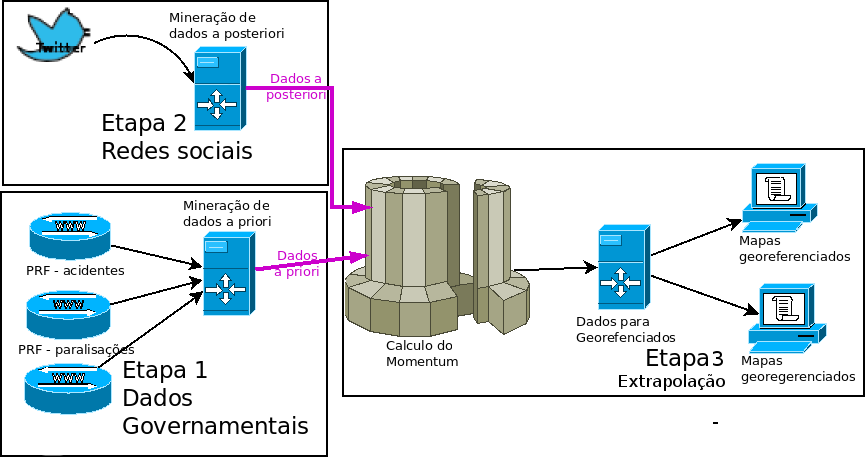
\includegraphics[width=135mm, height=75	mm]{Figuras/Metodologia/metodologiaGeral2.png}\\
\tiny Fonte: autor
\end{figure}

\section{Reflexão sobre as tecnologias utilizadas no modelo preditivo}\label{result}

Na fase de transformação de dados, da primeira etapa, onde são criadas novas variáveis, a proximidade entre as
bases heterogêneas foi conseguida utilizando regras de indução da lógica proposicional \cite{NorvigRussel2004}.
Nesta pesquisa, bases heterogêneas foram integralizadas em um único grande conjunto de dados, o ``data set''. As variáveis desse ``data set'' foram consideradas variáveis independentes, e preservadas aquelas com maior relevância ou as que continham a maior quantidade de conhecimento embutido, descoberto pelo cálculo da entropia e correlação linear. Foram também construídas novas variáveis, nas bases onde não havia correspondência, respeitando a lógica do negócio.\\
A tabela a seguir descreve as variáveis originais na base de dados de acidentes da PRF.

\begin{table}[htbp!]
	\centering
	\caption{Variáveis transformadas} 
	\begin{tabular}{r|l} \hline
		KM & Numeração do quilômetro arredondada \\
		BR & Nome da BR \\
		Condição Pista & Condição da pista: seca, molhado, ... \\
		Restrição de Visibilidade & Restrição de visibilidade: inexistente, neblina, .., outros \\
		Tipo Acidente & Tipo de Acidente: atropelamento, colisão lateral,..\\
		Causa Acidente & A possível causa do acidente: Falta de atenção, ... \\
		Traçado Via & Tipo de traçado da via: reta, curva, cruzamento, ... \\
		Tipo veículo & Tipo de veículo envolvido no acidente \\
		Dia da Semana & dia em que ocorreu o acidente\\
		Hora & que ocorreu o acidente/ocorrência no formato hh/mm/ss \\
		Qtd Mortos & Quantidade de mortos envolvidos \\
		Gravidade & Quantidade de acidentes graves \\
		Período & turno do dia em que se deu a ocorrência \\
	\end{tabular}
\end{table}
 

\pagebreak

\section{Extração do conhecimento - KDD}

O processo de descoberta do conhecimento iniciou-se com a coleta das bases de dados de acidentes da PRF. Optamos por coletar os dados dessa base diretamente na fonte,
ou seja dos servidores da PRF. Tais dados nos foram cedidos após alguns procedimentos burocráticos de praxe (ver anexos). Essa escolha foi motivada para tentar
mitigar o problema da qualidade dos dados. No artigo ``Uma análise da qualidade dos dados relativos aos boletins de ocorrências das rodovias federais para o processo de Mineração de Dados'' COSTA, BERNARDINI, LIMA et al \cite{Costa2015} destacam a não padronização e não aceitação dos dados pela comunidade internacional. EAVES, D. \cite{Eaves} sugere que os dados sejam disponibilizados da maneira como foram coletados.

A PRF tem ao menos duas bases \footnote{Somente mencionamos bases de dados que interessaram à essa pesquisa.} de dados referentes às ocorrências nas rodovias BRs. A base de acidentes rodoviários e a base de intervenções que guarda as ocorrências que paralisaram as rodovias, tais como: protestos ou paralisações dessa natureza, feitos pelas pessoas que vivem no entorno das rodovias.

Para traçar um painel da diversidade das rodovias pernambucanas, foi efetuado a priori uma classificação através do algoritmo Árvore de Decisão e comparado com o classificador Naïve Bayes. Mediu-se a acurácia dos classificadores, comparando-se uma técnica algorítmica com a outra. A variável ``BRajustada'' mostrou ser a melhor variável para exprimir o nó raiz da Árvore de Decisão. Isso porque classificou os dados com o maior número de verdadeiros positivos e menor número de falsos positivos, muitos iguais a zero, obtendo curvas ROC com índices acima de 0.90. O Naïve Bayes também obteve índices de acurácia próximos a este, quando utilizado com o mesmo procedimento.

Foram construídas matrizes dos resultados da classificação e predição, chamadas ``Matriz de Mortos'' e ``Matriz de Gravidade''. As matrizes de mortos refletem a quantidade de óbitos ocorridos em cada hora do dia, em determinado quilômetro da rodovia, contemplando, assim, duas dimensões (ver imagem a seguir). Foi estabelecida uma terceira dimensão para detalhar os dias da semana, uma vez que a utilização da rodovia tem características diferentes nos dias de semana e fins de semana. 

\pagebreak

\begin{figure}
\centering
\caption{Matriz de Mortos 2D}
\label{fig:MatrizMortos2D}
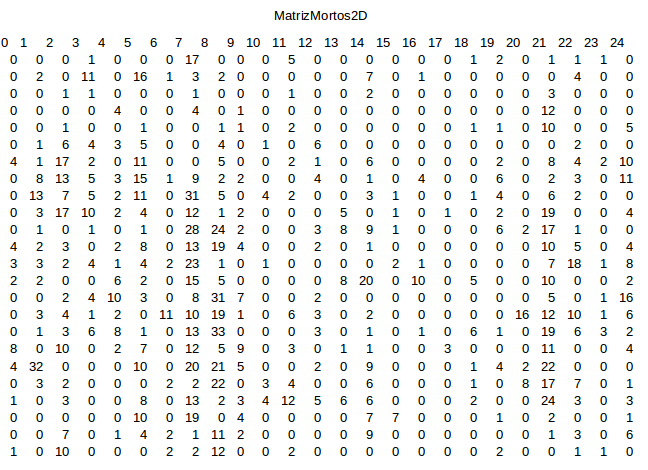
\includegraphics[width=110mm, height=65mm]{Figuras/Metodologia/MatrizMortos2D}\\
\tiny Fonte: Autor
\end{figure}

O exemplo acima apresenta as ocorrências na BR 101, onde as linhas representam as 24 horas do dia (0-23 horas) e as colunas representam cada km da rodovia, no caso dessa matriz, 214 km (0-213) para a BR 101. 

%\pagebreak

\begin{figure}[htbp!]
\centering
\caption{Km 70, BR 101 (Sul) Pernambuco}
\label{fig:Km70BR101}
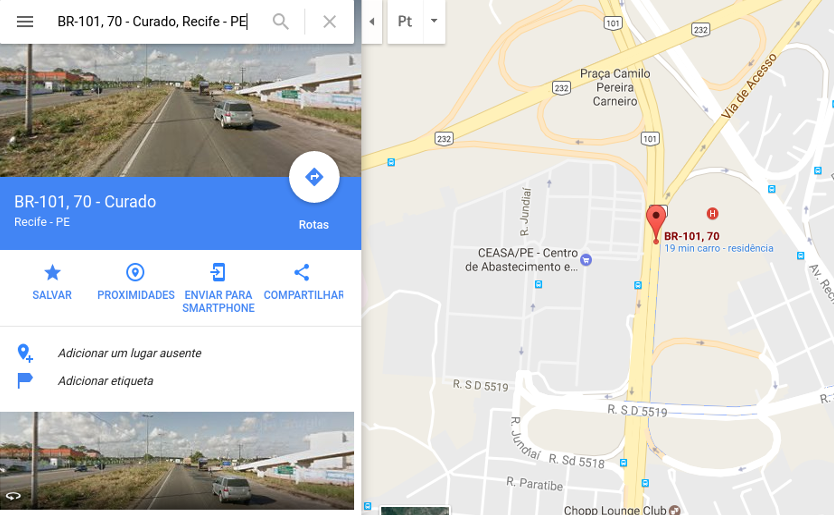
\includegraphics[width=110mm, height=65mm]{Figuras/Metodologia/Km70BR101}\\
\tiny Fonte: Google Maps
\end{figure}


O local com maior número de óbitos é no Km 70, Br 101 (sul), próximo à Ceasa

\pagebreak

As matrizes de mortos foram propostas com o objetivo de estimar o tempo de paralização da rodovia. Todavia, nem sempre um acidente com mortos implica em maior tempo de paralisação. Por exemplo, uma colisão que envolva muitos veículos, ainda que não houvesse óbitos, pode criar um maior constrangimento na rodovia do que, por exemplo, um atropelamento que tenha projetado a vítima para fora da pista. Em virtude disso, foram criadas as matrizes de gravidade, que contemplaram a maioria das variáveis transformadas, descritas anteriormente, resultando numa equação que integrou todos os fatores relacionados a uma ocorrência na rodovia. O exemplo a seguir representa uma Matriz de Gravidade 3D da BR 101. As linhas contemplam as 24 horas (0-23 horas); as colunas referem-se aos quilômetros da rodovia (0-213); e a terceira dimensão (que não aparece nessa imagem), os dias da semana (1 - segunda-feira... 7 - domingo). 

\begin{figure}
\centering
\caption{Matriz de Gravidade 3D}
\caption{}
\label{fig:MatrizGravidade3D2}
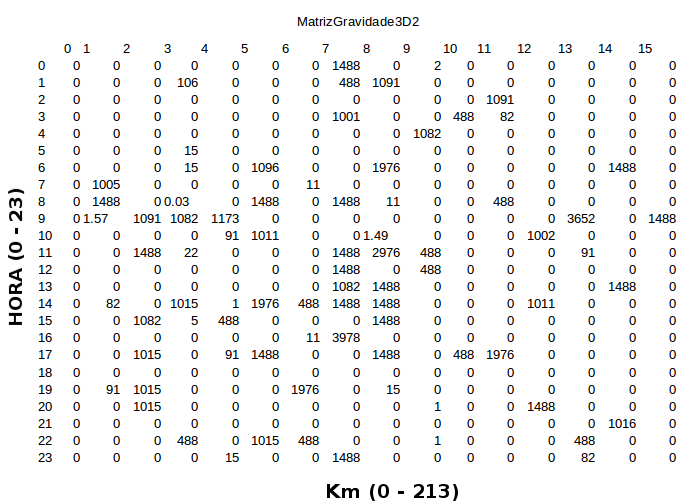
\includegraphics[width=0.7\linewidth]{Figuras/Metodologia/MatrizGravidade3D2}\\
\tiny Fonte: autor
\end{figure}

A equação que gera a Matriz de Gravidade foi proposta da seguinte forma: 

\begin{equation}
ProbAcid_{101} = (RestVisibi + CondPista + TracadoVia) *  Erro_{101} + Gravidade
\end{equation} 

Ainda sobre as matrizes - Mortos e Gravidade - a primeira contempla o número absoluto de óbitos que ocorreu em cada local da rodovia em todo o período contemplado na base de dados da PRF. A matriz de gravidade, por sua vez, apresenta cada uma das variáveis como uma probabilidade de ocorrência (ver equação). A variável ``gravidade'' é binária, sendo o valor 1 para ocorrência de óbito em determinado local e 0 para ausência de óbito. O ``Erro'' descrito na equação configura-se como um ajuste aos termos que aparecem entre parênteses, e foi utilizado com base na técnica ensemble, que afirma que o produto de dois classificadores resulta em um valor mais preciso.    



\pagebreak

\section{Arco cibernético com dados do Twitter}

Os dados do Twitter permitem uma busca imediata por novas informações que poderão ser confrontadas com o 
modelo preditivo, aumentando o nível de confiança deste. Com isso, as informações construirão um Arco cibernético. Segundo Wiener (1948), novas informações permitem realimentação aos sistemas, com maior potencial adaptativo, como pode ser visto nos exemplos de tweets identificados nessa pesquisa: no trecho da Br 101, na altura do km 5, no 
Município de Goiana, um utilizador do twitter publicou que a comunidade que mora no entorno dessa localidade fará um protesto nas primeiras horas do dia seguinte, devido a um  
atropelamento ocorrido na BR; ou a PRF publicou que o km 80 da Br 232, na altura do Município de Gravatá, será interditada no dia seguinte, por 2h, para 
remoção/explosão de rochas.

No entanto, quando as informações provenientes do modelo de predição entrarem em conflito com as informações 
provenientes das redes sociais \footnote{O sistema de predição é baseado em cálculos probabilísticos}, para estes casos a decisão de qual ação a ser tomada sempre estará ``nas mãos'' do agente, do observador ou do utilizador.

As informações das redes sociais que comporão o arco cibernético não deverão retroalimentar o modelo de predição já construído, pois o fluxo decisório já foi tomado pelo observador. Os dados a posteriori não servem para um modelo de predição, uma vez que enviesam o sistema preditivo.

\begin{figure}[ht]
	\centering
	\caption{O arco cibernético com o Twitter}
	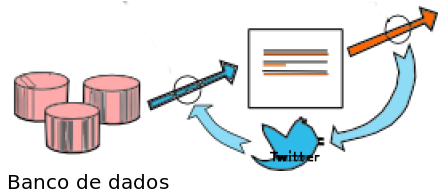
\includegraphics[width=90mm, height=45mm]{Figuras/Metodologia/ArcoCibernetico.png}\\
	\tiny Fonte: autor
\end{figure}

\pagebreak

\section{Extrapolação para georreferenciamento}

Os pontos críticos das matrizes geradas (de morte ou de gravidade) constituem-se como marcadores no mapa, que deverão ser levados em conta pelos utilizadores quando estiverem passando pelo local referenciado, conforme imagem a seguir.

\begin{figure}[ht]
	\centering
	\caption{Etapas da metodologia}
	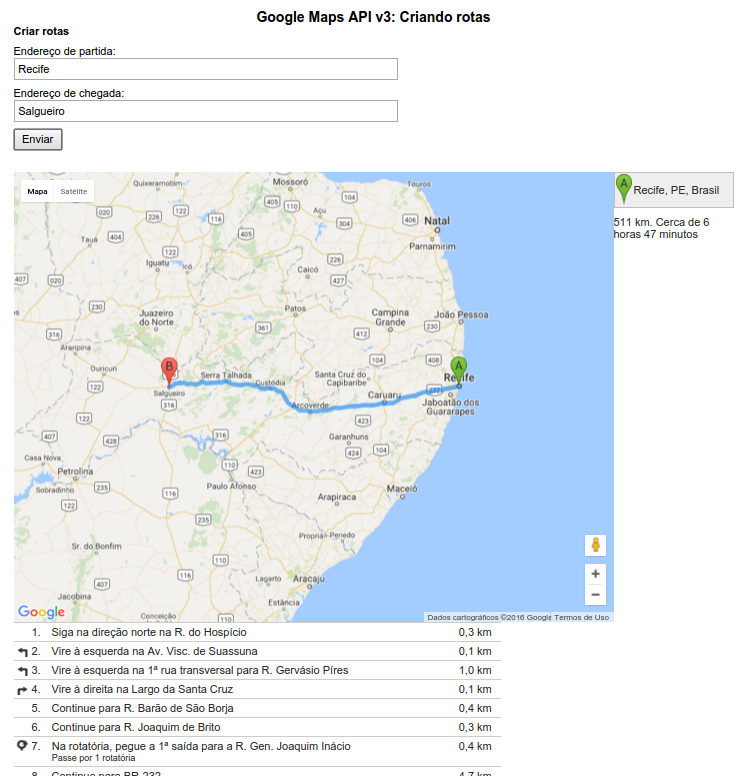
\includegraphics[width=150mm, height=130mm]{Figuras/Cronograma/GoogleMaps.png}\\
	\tiny Fonte: Google Maps
\end{figure}

O capítulo a seguir contemplará os resultados encontrados após a execução de todas as fases aqui apresentadas.


